\documentclass{article}



% This document contains the TikZ-header for all our LaTeX-computations.
% It especially contains all global graphic parameters.

\usepackage{amsmath, amssymb, amsfonts} % Standard Math-stuff

\usepackage{tikz}
\usetikzlibrary{calc}
\usetikzlibrary{positioning}
\usetikzlibrary{shapes}
\usetikzlibrary{patterns}

% Define a text=none option for nodes that ignores the given text, from
% https://tex.stackexchange.com/questions/59354/no-text-none-in-tikz
\makeatletter
\newif\iftikz@node@phantom
\tikzset{
  phantom/.is if=tikz@node@phantom,
  text/.code=%
    \edef\tikz@temp{#1}%
    \ifx\tikz@temp\tikz@nonetext
      \tikz@node@phantomtrue
    \else
      \tikz@node@phantomfalse
      \let\tikz@textcolor\tikz@temp
    \fi
}
\usepackage{etoolbox}
\patchcmd\tikz@fig@continue{\tikz@node@transformations}{%
  \iftikz@node@phantom
    \setbox\pgfnodeparttextbox\hbox{}
  \fi\tikz@node@transformations}{}{}
\makeatother

% Now we define the global styles
% The global styles are defined nestedly. You have to give your tikzpicture
% the global options [vertexStyle, edgeStyle, faceStyle] to activate them.
% 
% You can disable labels by using the option nolabels, i.e. 
% vertexStyle=nolabels to deactivate vertex labels.
%
% If you want to have a specific style for your picture, you can also use
% this specific meta-style instead of the general style. For example if you
% want to use double edges in one single picture - no matter the style of
% the rest of the document - you can use edgeDouble instead of edgeStyle.
%
% To set the default style, modify the vertexStyle/.default entry.

% Vertex styles
\tikzset{ 
    vertexNodePlain/.style = {fill=gray, shape=circle, inner sep=0pt, minimum size=2pt, text=none},
    vertexPlain/labels/.style = {
        vertexNode/.style={vertexNodePlain},
        vertexLabel/.style={gray}
    },
    vertexPlain/nolabels/.style = {
        vertexNode/.style={vertexNodePlain},
        vertexLabel/.style={text=none}
    },
    vertexPlain/.style = vertexPlain/#1,
    vertexPlain/.default=labels
}
\tikzset{
    vertexNodeNormal/.style = {fill=blue, shape=circle, inner sep=0pt, minimum size=4pt, text=none},
    vertexNormal/labels/.style = {
        vertexNode/.style={vertexNodeNormal},
        vertexLabel/.style={blue}
    },
    vertexNormal/nolabels/.style = {
        vertexNode/.style={vertexNodeNormal},
        vertexLabel/.style={text=none}
    },
    vertexNormal/.style = vertexNormal/#1,
    vertexNormal/.default=labels
}
\tikzset{
    vertexNodeBall/.style = {shape=circle, ball color=orange, inner sep=2pt, outer sep=0pt, minimum size=3pt, font=\tiny},
    vertexBall/labels/.style = {
        vertexNode/.style={vertexNodeBall, text=black},
        vertexLabel/.style={text=none}
    },
    vertexBall/nolabels/.style = {
        vertexNode/.style={vertexNodeBall, text=none},
        vertexLabel/.style={text=none}
    },
    vertexBall/.style = vertexBall/#1,
    vertexBall/.default=labels
}
\tikzset{ 
    vertexStyle/.style={vertexNormal=#1},
    vertexStyle/.default = labels
}


% 1) position of the vertex
% 2) relative position of the node
% 3) name of the vertex
\newcommand{\vertexLabelR}[3]{
    \node[vertexNode] at (#1) {#3};
    \node[vertexLabel, #2] at (#1) {#3};
}
% 1) position of the vertex
% 2) absolute position of the node
% 3) name of the vertex
\newcommand{\vertexLabelA}[3]{
    \node[vertexNode] at (#1) {#3};
    \node[vertexLabel] at (#2) {#3};
}


% Edge styles
% If you have trouble with the double-lines overlapping, this might (?) help:
% https://tex.stackexchange.com/questions/288159/closing-the-ends-of-double-line-in-tikz
\newcommand{\edgeLabelColor}{blue!20!white}
\tikzset{
    edgeLineNone/.style = {draw=none},
    edgeLineNone/.default=black,
    edgeNone/labels/.style = {
        edge/.style = {edgeLineNone=##1},
        edgeLabel/.style = {fill=\edgeLabelColor}
    },
    edgeNone/nolabels/.style = {
        edge/.style = {edgeLineNone=##1},
        edgeLabel/.style = {text=none}
    },
    edgeNone/.style = edgeNone/#1,
    edgeNone/.default = labels
}
\tikzset{
    edgeLinePlain/.style={line join=round, draw=#1},
    edgeLinePlain/.default=black,
    edgePlain/labels/.style = {
        edge/.style={edgeLinePlain=##1},
        edgeLabel/.style={fill=\edgeLabelColor}
    },
    edgePlain/nolabels/.style = {
        edge/.style={edgeLinePlain=##1},
        edgeLabel/.style={text=none}
    },
    edgePlain/.style = edgePlain/#1,
    edgePlain/.default = labels
}
\tikzset{
    edgeLineDouble/.style = {thin, double=#1, double distance=.6pt, line join=round},
    edgeLineDouble/.default=gray!90!white,
    edgeDouble/labels/.style = {
        edge/.style = {edgeLineDouble=##1},
        edgeLabel/.style = {fill=\edgeLabelColor}
    },
    edgeDouble/nolabels/.style = {
        edge/.style = {edgeLineDouble=##1},
        edgeLabel/.style = {text=none}
    },
    edgeDouble/.style = edgeDouble/#1,
    edgeDouble/.default = labels
}
\tikzset{
    edgeStyle/.style = {edgePlain=#1},
    edgeStyle/.default = labels
}

% Face styles
% Here we have an exception - the style face is always defined.
% 
\newcommand{\faceColorY}{yellow!60!white}   % yellow
\newcommand{\faceColorB}{blue!60!white}     % blue
\newcommand{\faceColorC}{cyan!60}           % cyan
\newcommand{\faceColorR}{red!60!white}      % red
\newcommand{\faceColorG}{green!60!white}    % green
\newcommand{\faceColorO}{orange!50!yellow!70!white} % orange

% define default face colour (and default swap colour)
\newcommand{\faceColor}{\faceColorY}
\newcommand{\faceColorSwap}{\faceColorC}

% define secondary default colours (to use in a single section)
\newcommand{\faceColorFirst}{green!40!white}
\newcommand{\faceColorSecond}{gray!15!white}
\newcommand{\faceColorThird}{red!17!white}
\newcommand{\faceColorFourth}{olive!20!white}

\tikzset{
    face/.style = {fill=#1},
    face/.default = \faceColor,
    faceY/.style = {face=\faceColorY},
    faceB/.style = {face=\faceColorB},
    faceC/.style = {face=\faceColorC},
    faceR/.style = {face=\faceColorR},
    faceG/.style = {face=\faceColorG},
    faceO/.style = {face=\faceColorO}
}
\tikzset{
    faceStyle/labels/.style = {
        faceLabel/.style = {}
    },
    faceStyle/nolabels/.style = {
        faceLabel/.style = {text=none}
    },
    faceStyle/.style = faceStyle/#1,
    faceStyle/.default = labels
}
\tikzset{ face/.style={fill=#1} }
\tikzset{ faceSwap/.code=
    \ifdefined\swapColors
        \tikzset{face=\faceColorSwap}
    \else
        \tikzset{face=\faceColor}
    \fi
}

% Sometimes we want to implement different behaviour for the generated 
% HTML-pictures (for example, shading is not supported in HTML).
% For that we define a macro to check whether we run the code with
% htlatex. The code comes from 
% https://tex.stackexchange.com/questions/93852/what-is-the-correct-way-to-check-for-latex-pdflatex-and-html-in-the-same-latex
\makeatletter
\edef\texforht{TT\noexpand\fi
  \@ifpackageloaded{tex4ht}
    {\noexpand\iftrue}
    {\noexpand\iffalse}}
\makeatother


\usepackage{hyperref}

\if\texforht
    \def\pgfsysdriver{pgfsys-tex4ht.def}
\fi
\usetikzlibrary{arrows, decorations.pathreplacing, calc, decorations.pathmorphing, shapes}

\usepackage{amssymb}

\begin{document}

\tikzset{
    test/ht/.style={shape=circle, fill=#1},
    test/normal/.style={shape=circle, ball color=#1},
    test/.code={
        \if\texforht\tikzset{test/ht=#1}\else\tikzset{test/normal=#1}\fi
    },
    neu/.style={test=#1, font=\small}
}

\begin{tikzpicture}
    \node[neu=green] at (0,0) {8};
\end{tikzpicture}

%\end{document}

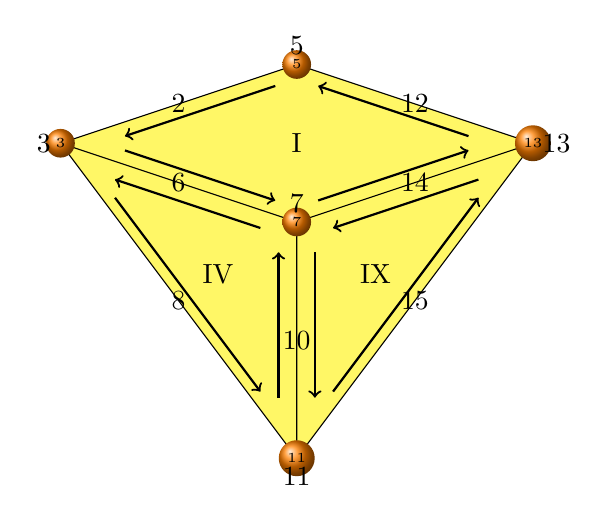
\begin{tikzpicture}[vertexBall,edgePlain=nolabels,faceStyle=nolabels]
    \def\orientation{1}
        \def\hor{3}
    \def\ver{1}
    \def\down{4}
    \coordinate (L) at (-\hor,0);
    \coordinate (R) at (\hor,0);
    \coordinate (U) at (0,\ver);
    \coordinate (D) at (0,-\ver);
    \coordinate (DD) at (0,-\down);

    \draw[face,edge]
        (L) -- node[edgeLabel] {2} (U) -- node[edgeLabel] {12} (R) -- (D) -- cycle
        (L) -- node[edgeLabel] {6} (D) -- (DD) -- node[edgeLabel] {8} cycle
        (D) -- node[edgeLabel] {10} (DD) -- node[edgeLabel] {15} (R) -- node[edgeLabel] {14} cycle;

    \node[faceLabel] at (0,0) {I};
    \node[faceLabel] at (barycentric cs:L=1,D=1,DD=1) {IV};
    \node[faceLabel] at (barycentric cs:D=1,R=1,DD=1) {IX};

    \foreach \p/\r/\n in {L/left/3, U/above/5, R/right/13, D/above/7, DD/below/11}{
        \vertexLabelR{\p}{\r}{\n}
    }

    \ifdefined\orientation
        % use barycentric coordinates with primary and secondary vertices
        % quadrangle, obtuse
        \def\qop{8}
        \def\qos{2}
        % quadrangle, acute
        \def\qap{8}
        \def\qas{2}
        % triangle, left
        \def\tlp{10}
        \def\tls{2}
        % triangle, mid
        \def\tmp{10}
        \def\tms{2}

        \draw[thick, ->] (barycentric cs:L=\qap,D=\qas,U=1) -- (barycentric cs:D=\qop,L=\qos,R=1);
        \draw[thick, ->] (barycentric cs:D=\qop,R=\qos,L=1) -- (barycentric cs:R=\qap,D=\qas,U=1);
        \draw[thick, ->] (barycentric cs:R=\qap,U=\qas,D=1) -- (barycentric cs:U=\qop,R=\qos,L=1);
        \draw[thick, ->] (barycentric cs:U=\qop,L=\qos,R=1) -- (barycentric cs:L=\qap,U=\qas,D=1);

        \draw[thick, ->] (barycentric cs:L=\tlp,DD=\tls,D=1) -- (barycentric cs:DD=\tlp,L=\tls,D=1);
        \draw[thick, ->] (barycentric cs:DD=\tlp,D=\tls,L=1) -- (barycentric cs:D=\tlp,DD=\tls,L=1);
        \draw[thick, ->] (barycentric cs:D=\tlp,L=\tls,DD=1) -- (barycentric cs:L=\tlp,D=\tls,DD=1);

        \draw[thick, <-] (barycentric cs:R=\tlp,DD=\tls,D=1) -- (barycentric cs:DD=\tlp,R=\tls,D=1);
        \draw[thick, <-] (barycentric cs:DD=\tlp,D=\tls,R=1) -- (barycentric cs:D=\tlp,DD=\tls,R=1);
        \draw[thick, <-] (barycentric cs:D=\tlp,R=\tls,DD=1) -- (barycentric cs:R=\tlp,D=\tls,DD=1);
    \fi

\end{tikzpicture}


\begin{tikzpicture}
    \foreach \i in {1,...,3}
        \coordinate (A\i) at (-0.5+\i, 0);

    \foreach \i in {1,2,3}
        \fill (A\i) circle (2pt);

\end{tikzpicture}


\end{document} 
